%Fiquemos com Deus e Nossa Senhora!
%Sao Jose de Cupertino rogai por nos!!
% ### Uses XeLaTeX ### %
% ### Needs beamer-master ### %
\documentclass[aspectratio=169]{beamer} %. Aspect Ratio 16:9

\usetheme{AI2} % beamerthemeSprace.sty
\usepackage[portuguese]{babel}
\usepackage[utf8]{inputenc}
\usepackage[T1]{fontenc}
\usepackage{ragged2e}

\DeclareMathOperator*{\argmin}{arg\,min}
\DeclareMathOperator*{\argmax}{arg\,max}

% DATA FOR FOOTER
\date{2021}
\title{- Regressão Logística}
\author{João Paulo Papa}
\institute{Advanced Institute for Artificial Intelligence (AI2)}

\begin{document}
% ####################################
% FIRST SLIDE 						:: \SliTit{This is the Title of the Talk}{A. B. Name}{Sprace}
% SUB-TITLE SLIDE 					:: \SliSubTit{<title>}{<explanation}
% SUB-SUB-TITLE SLIDE				:: \SliSubSubTit{<title>}{<explanation}
% SLIDE WITH TITLE 					:: \SliT{Title}{Content}
% SLIDE NO TITLE 						:: \Sli{Content} 
% SLIDE DOUBLE COLUMN WITH TITLE 	:: \SliDT{Title}{First Column}{Second Column}
% SLIDE DOUBLE COLUMN NO TITLE 		:: \SliD{First Column}{Second Column}
% SLIDE ADVANCED WITH TITLE 			:: \SliAdvT{Title}{Content}
% SLIDE ADVANCED NO TITLE 			:: \SliAdv{Content}
% SLIDE ADVANCED DOUBLE WITH TITLE 	:: \SliAdvDT{Title}{First Column}{Second Column}
% SLIDE ADVANCED DOUBLE NO TITLE 	:: \SliAdvD{First Column}{Second Column}
% SLIDE BLACK						:: \Black{ <Content> }
% SLIDE WHITE						:: \White{ <Content> }
% ITEMIZATION 						:: \begin{itemize}  \iOn{First} \iTw {Second} \iTh{Third} \end{itemize}
% COMMENT TEXT				 		:: \note{<comment>}
% SECTION 							:: \secx{Section} | \secxx{Sub-Section}
% BOLD SPRACE COLOR				:: \bfs{<text>}
% TABLE OF CONTENT					:: \tocitem{<title>}{<content>}
% LEFT ALIGN EQUATION				:: \begin{flalign*}  & <equation> &   \end{flalign*}
% CENTER ALIGN EQUATION	S			:: \begin{gather*} <equations>  \end{gather*}
% SLASH								:: \slashed{<>}
% BAR								:: \barr{<letter>} instead of \bar{<letter>}
% THEREFORE						:: use \portanto (larger and bold}
% 2 or 3 MATH SYMBOLS				:: \overset{<up>}{<down>} &  \underset{<below>}{\overset{<above>}{<middle>}}  
% INSERT TEXT IN FORMULA			:: \ins{<text>}
% EXERCISE							:: \exe{<exercise #>}{<exercise text>}
% SUGGESTED READING BOX			:: \sug{<references>}
% CITATION							:: \cittex{<citation>}
% CITATION DOUBLE COLUMN 			:: \cittexD{<citation>}
% TEXT POSITION						:: \texpos{<Xcm>}{<Ycm>}{<text>} origin = center of slide : x right | y down
% REFERENCE AT BOTTOM  S/D SLIDE		:: \refbotS{<reference>} \refbotD{<reference>}
% HIDDEN SLIDE						:: \hid
% COLOR BOX 						:: \blu{blue} + \red{rec} + \yel{yellow} + \gre{green} + \bege{beige}
% FRAME 							:: \fra{sprace} \frab{blue} \frar{red} + \fray{yellow} + \frag{green}		
% FIGURE 							:: \img{X}{Y}{<scale>}{Figure.png} 
% FIGURE							:: \includegraphics[scale=<scale>]{Figures/.png}
% FIGURE DOUBLE SLIDE NO TITLE		::  \img{-4}{0.5}{<scale>}{Figure.png} % Image 1st half
%									::  \img{4}{0.5}{<scale>}{Figure.png} % Image 2nd half
% FIGURE DOUBLE SLIDE WITH TITLE		::  \img{-4}{0}{<scale>}{Figure.png} % Image 1st half
%									::  \img{4}{0}{<scale>}{Figure.png} % Image 2nd half
% INCLUDING SWF (Flash)				:: \usepackage{media9} and \includemedia >> USE ACROBAT <<
%%%%%%%%%%%%%%%%%%%%%%%%%%%%%%%%%%%%%%%%%%%%%%%%%%
% ###############################################################################
% FIRST SLIDE
\SliTit{Regressão Logística}{Advanced Institute for Artificial Intelligence -- AI2}{https://advancedinstitute.ai}
%%%%%%%%%%%%%%%%%%%%%%%%%%%%%%%%%%%%%%%%%%%%%%%%%%
% ###############################################################################
% SLIDE SUB-TITLE
%\SliSubTit{Sub-Title}{Description}{}
%%%%%%%%%%%%%%%%%%%%%%%%%%%%%%%%%%%%%%%%%%%%%%%%%%
% ###############################################################################
%\SliSubSubTit{Sub-Sub-Title}{Description}
 %%%%%%%%%%%%%%%%%%%%%%%%%%%%%%%%%%%%%%%%%%%%%%%%%%


\SliT{Introdução}{

\justifying Existem problemas para os quais desejamos estimar a \textbf{classe} (rótulo) de uma determinada amostra com base no seu conjunto de dados de entrada, isto é, as \textbf{características} do seu problema.

\justifying Problemas de classificação são similares aos de regressão pois desejamos aprender uma função que, dada uma entrada, estime um valor de saída. A diferença é que nossa saída será mapeada para uma \textbf{probabilidade} (\emph{soft classification}) ou \textbf{rótulo} (\emph{hard classification}) da amostra.

\justifying A técnica de Regressão Logística é uma das mais utilizadas na literatura, principalmente por ser simples e dar bons resultados em diversas situações. Ela tem esse nome pelo fato de estimar a probabilidade de uma dada amostra pertencer à uma classe em específico. Portanto, é uma técnica de classificação do tipo \emph{soft}.
}

\Sli{
\justify \underline{Definição do problema:} seja um conjunto de dados ${\cal X}= \{(\boldsymbol{x}_1,y_1),(\boldsymbol{x}_2,y_2),\ldots,(\boldsymbol{x}_z,y_z)\}$ tal que $\boldsymbol{x}_i\in\mathbb{R}^{n+1}$ corresponde ao dado de entrada e $y_i\in[0,1]$ denota o seu respectivo valor de saída. Temos, ainda, que ${\cal X}$ pode ser \textbf{particionado} da seguinte forma: ${\cal X} = {\cal X}^1\cup {\cal X}^2$, em que ${\cal X}^1$ e ${\cal X}^2$ denotam os conjuntos de dados de \textbf{treinamento} e \textbf{teste}, respectivamente. Nosso objetivo é, dado o conjunto de treinamento, aprender uma função $h:\mathbb{R}^{n+1}\rightarrow[0,1]$ que consiga estimar a probabilidade de uma amostra pertencer à uma dada classe. Por que usar uma função logística (sigmoide)?
}

\Sli{
A Função Logística possui algumas propriedades interessantes com a seguinte formulação:

\begin{equation}
	g(a)=\frac{1}{1+e^{-a}},
\end{equation}
tal que $g(a)\in[0,1]$.
\begin{center}
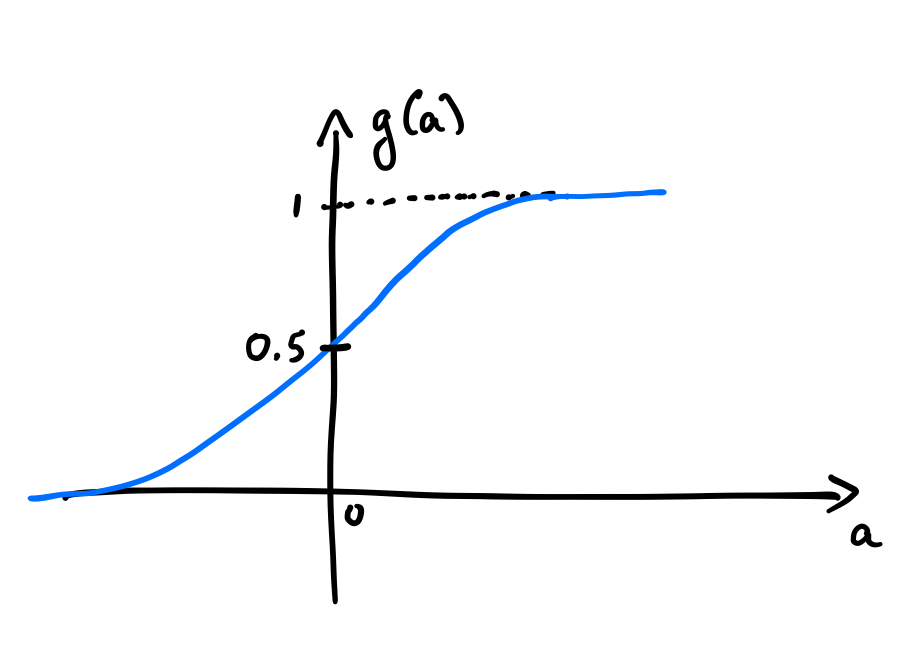
\includegraphics[scale=0.17]{./figs/Regressao_Logistica_Fig1.png}\hspace{1cm}
\end{center}
}

\Sli{
Como funciona o Regressor Logístico? Dado que queremos obter uma saída $h_{\boldsymbol{w}}(\boldsymbol{x})\in[0,1]$, basta modificarmos nossa entrada na Equação 1 como segue:

\begin{align}\nonumber
	h_{\boldsymbol{w}}(\boldsymbol{x}) &= g(\boldsymbol{w}^T\boldsymbol{x})\\
	&= \frac{1}{1+e^{-\boldsymbol{w}^T\boldsymbol{x}}}.
\end{align}
Agora, o termo $\boldsymbol{w}^T\boldsymbol{x}$ é chamado de \textbf{função base}.

\begin{minipage}{0.49\textwidth}
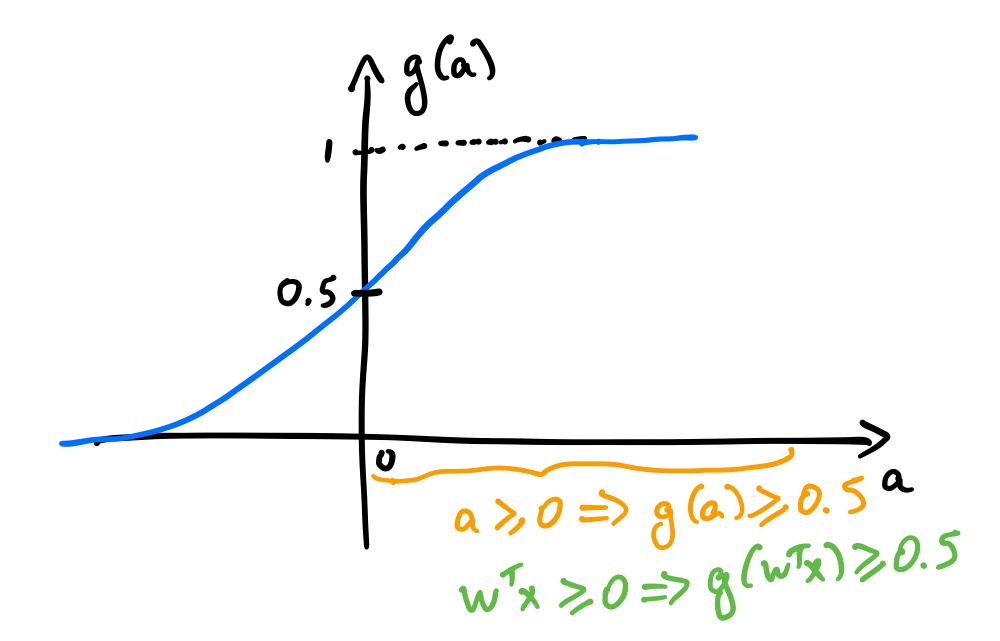
\includegraphics[scale=0.17]{./figs/Regressao_Logistica_Fig2.png}
\end{minipage}%%% to prevent a space
\begin{minipage}{0.37\textwidth}
Na prática, queremos que $h_{\boldsymbol{w}}(\boldsymbol{x})\geq 0.5$ quando $\boldsymbol{w}^T\boldsymbol{x}\geq 0$. De maneira análoga, temos que $h_{\boldsymbol{w}}(\boldsymbol{x})< 0.5$ quando $\boldsymbol{w}^T\boldsymbol{x}< 0$.
\null
\par\xdef\tpd{\the\prevdepth}
\end{minipage}
}	

\Sli{
\justify Suponha que tenhamos a seguinte situação, em que $h_{\boldsymbol{w}}(\boldsymbol{x})=g(\boldsymbol{w}^T\boldsymbol{x})$ e $\boldsymbol{w} = [-3\ 1\ 1]$. Queremos atribuir $y=1$ se $\boldsymbol{w}^T\boldsymbol{x}> 0$, ou seja, se $-3+x^1+x^2>0\Rightarrow x^1+x^2>3$. De maneira análoga, queremos atribuir $y=0$ se $\boldsymbol{w}^T\boldsymbol{x}< 0$, ou seja, se $-3+x^1+x^2<0\Rightarrow x^1+x^2<3$.

\begin{center}
\begin{minipage}{0.37\textwidth}
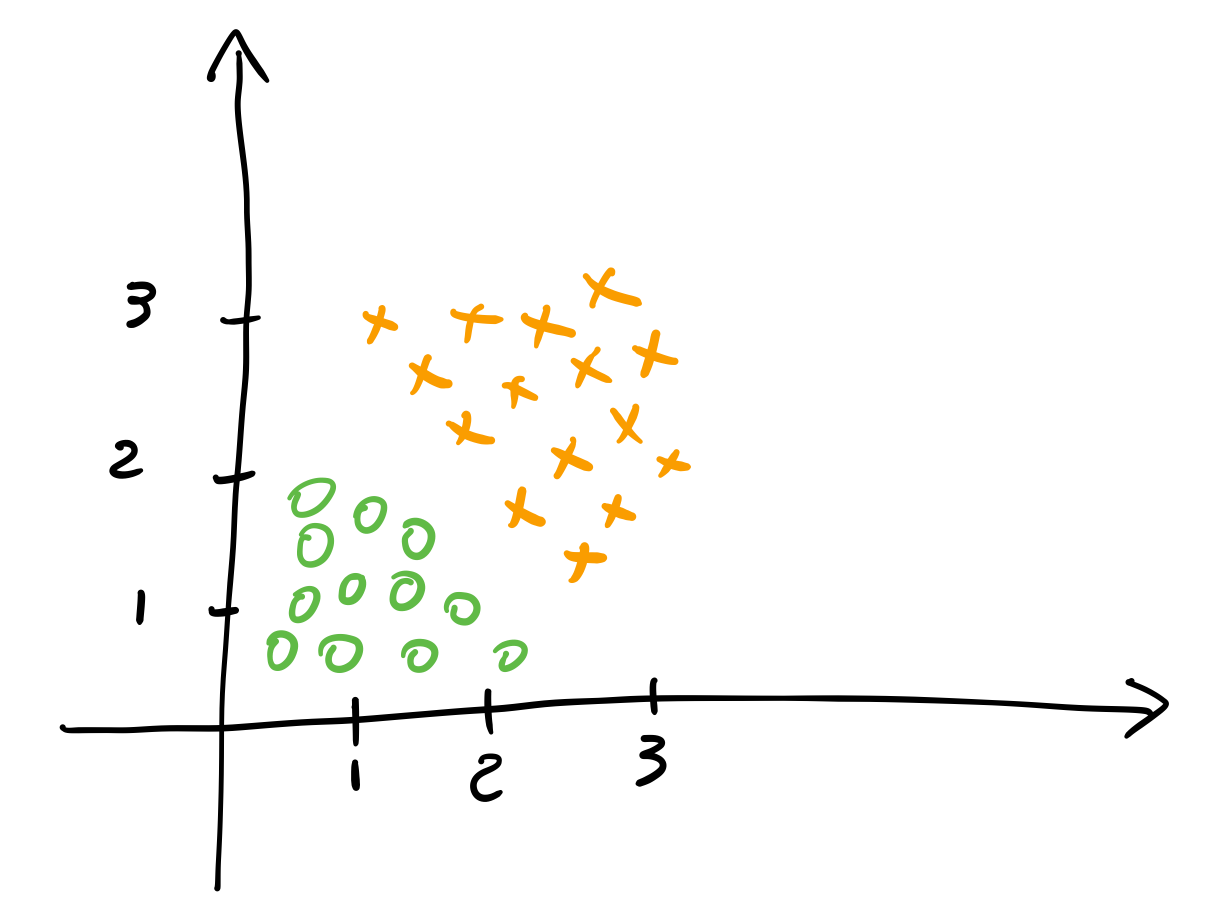
\includegraphics[scale=0.117]{./figs/Regressao_Logistica_Fig3.png}
\end{minipage}%%% to prevent a space
\begin{minipage}{0.37\textwidth}
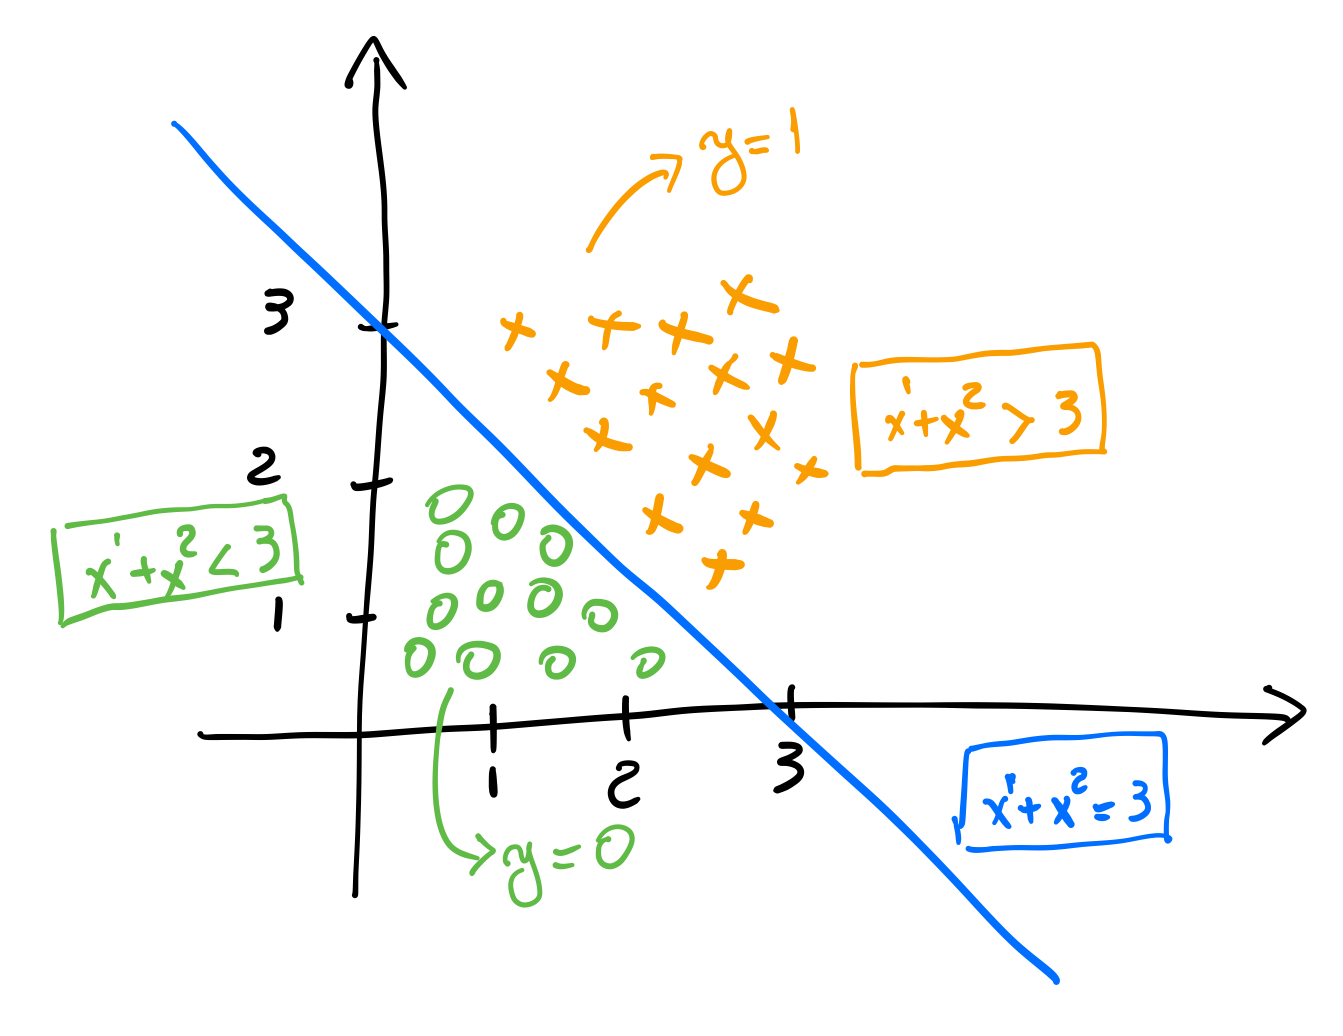
\includegraphics[scale=0.117]{./figs/Regressao_Logistica_Fig4.png}
\end{minipage}%%% to prevent a space
\end{center}
}	

\Sli{
\justify Suponha agora outra situação, em que $h_{\boldsymbol{w}}(\boldsymbol{x})=g(w_0+w_1x^1+w_2x^2+w_3(x^1)^2+w_4(x^2)^2)$ e $\boldsymbol{w} = [-1\ 0\ 0\ 1\ 1]$. Queremos atribuir $y=1$ se $-1+(x^1)^2+(x^2)^2>0\Rightarrow (x^1)^2+(x^2)^2>1$. De maneira análoga, queremos atribuir $y=0$ se $1+(x^1)^2+(x^2)^2<0\Rightarrow (x^1)^2+(x^2)^2<1$.
\vspace{-0.5cm}
\begin{center}
\begin{minipage}{0.37\textwidth}
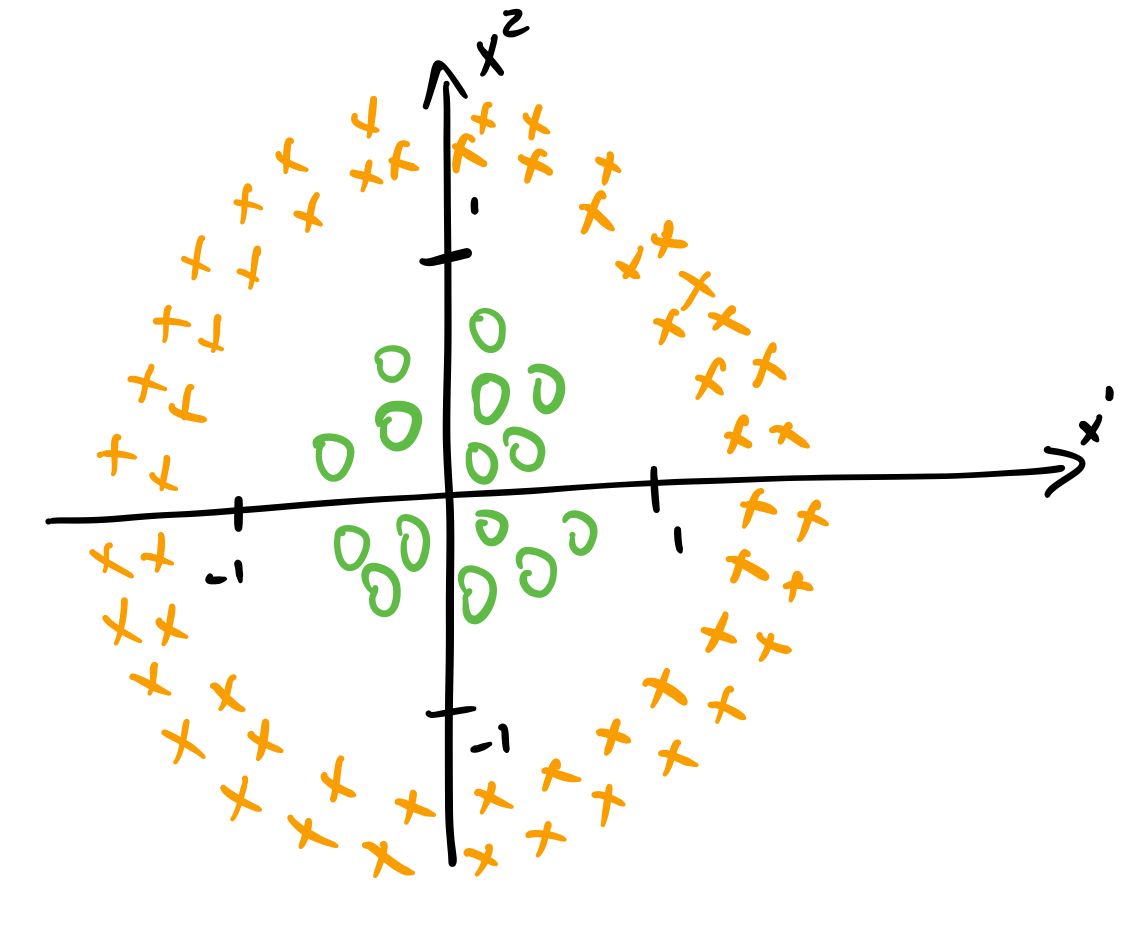
\includegraphics[scale=0.117]{./figs/Regressao_Logistica_Fig5.png}
\end{minipage}%%% to prevent a space
\begin{minipage}{0.37\textwidth}
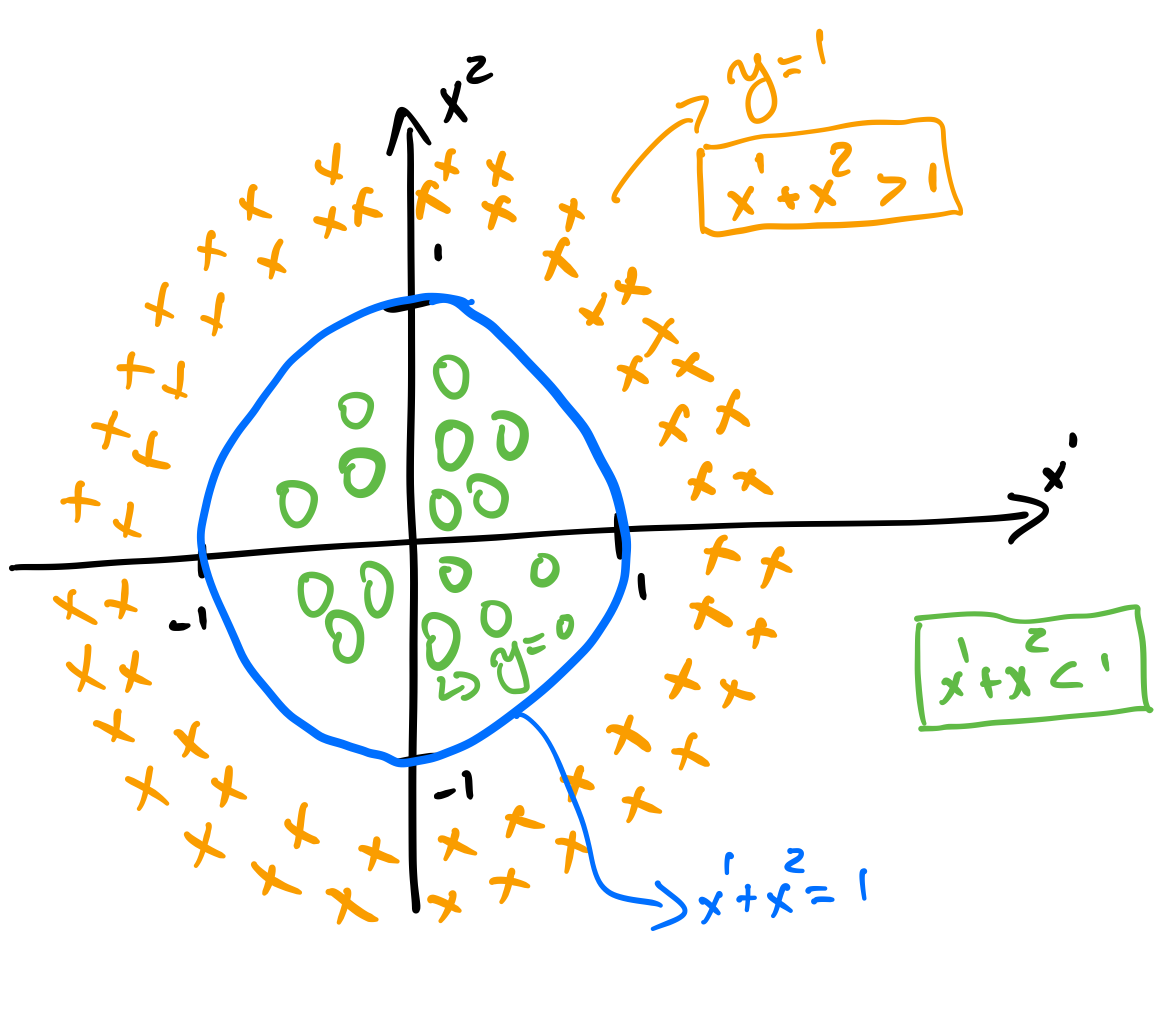
\includegraphics[scale=0.117]{./figs/Regressao_Logistica_Fig6.png}
\end{minipage}%%% to prevent a space
\end{center}
Desta forma, podemos notar que, dependendo da função base escolhida, diferentes superfícies de separação podem ser obtidas. Usualmente, quanto maior o grau do polinômio, mais complexa será a sua superfície.
}

\Sli{
Assim sendo, temos as seguintes informações até o momento:

\begin{itemize}
	\item Função hipótese: $h_{\boldsymbol{w}}(\boldsymbol{x}) = \frac{1}{1+e^{-\boldsymbol{w}^T\boldsymbol{x}}}$.
	\item Função base: $f_{\boldsymbol{w}}(\boldsymbol{x})=\boldsymbol{w}^T\boldsymbol{x}$ (padrão).
	\item Função de custo: ?
\end{itemize}
Por que não é interessante utilizar MSE como função de custo para o Regressor Logístico?
}

\Sli{
Temos dois problemas principais com MSE quando usamos a técnica de Regressão Logística:

\begin{enumerate}
	\item Suponha que o rótulo verdadeiro de uma amostra $\boldsymbol{x}\in{\cal X}$ qualquer seja $y=1$, e nosso classificador tenha resultado como saída $h_{\boldsymbol{w}}(\boldsymbol{x}) = 0$. Neste caso (para $m=1$), temos que $J(\boldsymbol{w}) = \frac{1}{2}(1-0)^2 = 0.5$. Note que essa é uma penalização muito pequena para um \textbf{erro} de classificação. Assim sendo, MSE não penaliza muito fortemente erros de classificação e pode levar a um aprendizado insuficiente.\\
	\item A função de custo MSE \textbf{não é convexa} para o Regressor Logístico (provado matematicamente).
\end{enumerate}
}

\Sli{
Vamos, então, definir uma nova função de custo que seja convexa. Nossa função será dividida, inicialmente, em duas partes:

\begin{equation}
	C(h_{\boldsymbol{w}}(\boldsymbol{x}), y) = \begin{cases}
                        -\log (h_{\boldsymbol{w}}(\boldsymbol{x})) \text{ se $y=1$} \\
                        -\log(1-h_{\boldsymbol{w}}(\boldsymbol{x})) \text{ se $y=0$}.
                    \end{cases}
\end{equation}

Vamos, agora, analisar as duas situações separadamente. Como primeiro caso, temos a situação em que $y=1$.

\begin{minipage}{0.49\textwidth}
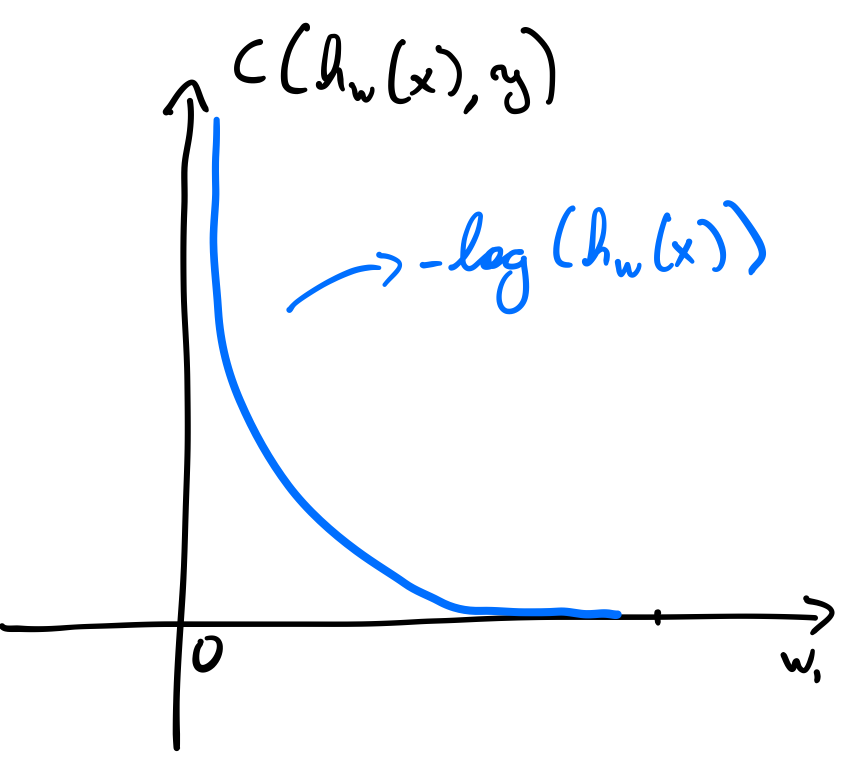
\includegraphics[scale=0.17]{./figs/Regressao_Logistica_Fig7.png}
\end{minipage}%%% to prevent a space
\begin{minipage}{0.37\textwidth}
Neste caso, quando temos um erro, ou seja, $h_{\boldsymbol{w}}(\boldsymbol{x}) = 0$, então $C(h_{\boldsymbol{w}}(\boldsymbol{x}), y) = -\log(0) = \infty$. No caso de um acerto, ou seja, $h_{\boldsymbol{w}}(\boldsymbol{x}) = 1$, temos que $C(h_{\boldsymbol{w}}(\boldsymbol{x}), y) = -\log(1) = 0$
\null
\par\xdef\tpd{\the\prevdepth}
\end{minipage}
}

\Sli{
A próxima situação ocorre quando $y=0$.

\begin{minipage}{0.49\textwidth}
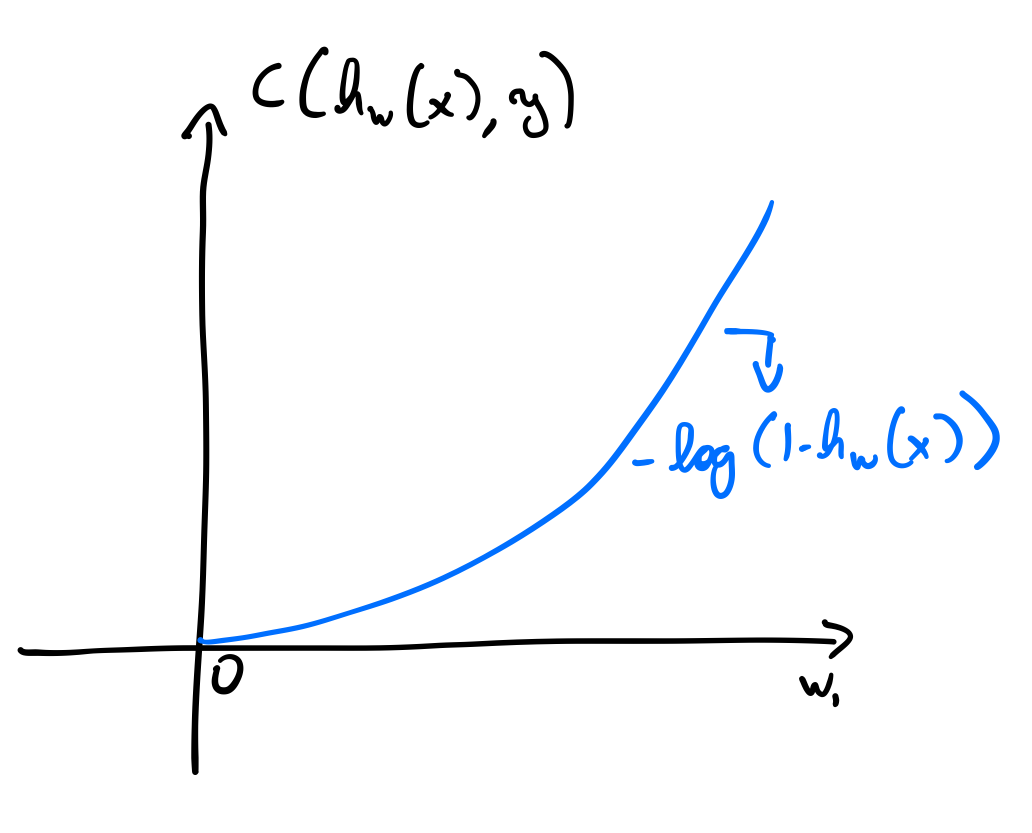
\includegraphics[scale=0.17]{./figs/Regressao_Logistica_Fig8.png}
\end{minipage}%%% to prevent a space
\begin{minipage}{0.37\textwidth}
Neste caso, quando temos um erro, ou seja, $h_{\boldsymbol{w}}(\boldsymbol{x}) = 1$, então $C(h_{\boldsymbol{w}}(\boldsymbol{x}), y) = -\log(1-1) = -\log(0) = \infty$. No caso de um acerto, ou seja, $h_{\boldsymbol{w}}(\boldsymbol{x}) = 0$, temos que $C(h_{\boldsymbol{w}}(\boldsymbol{x}), y) = -\log(1-0) = -\log(1) = 0$.
\null
\par\xdef\tpd{\the\prevdepth}
\end{minipage}
}

\Sli{
Podemos escrever a Equação 3 agrupando as duas situações descritas anteriormente:

\begin{equation}
	C(h_{\boldsymbol{w}}(\boldsymbol{x}), y) = \textcolor{blue}{-y\log(h_{\boldsymbol{w}}(\boldsymbol{x}))}\textcolor{red}{-(1-y)log(1-h_{\boldsymbol{w}}(\boldsymbol{x}))}.
\end{equation}
\justify Quando \textcolor{blue}{$y=1$}, termo vermelho é zerado e a equação acima torna-se a Equação 3 para este caso. Por outro lado, quando \textcolor{red}{$y=0$}, termo azul é zerado e a equação acima torna-se a Equação 3 para este caso.
}

\Sli{
A nossa função de custo final para o Regressor Logístico é dada por:

\begin{align}\nonumber
	J(\boldsymbol{w}) &= \frac{1}{m} \sum_{i=1}^m C(h_{\boldsymbol{w}}(\boldsymbol{x}_i), y_i)\\
	&= \frac{1}{m} \sum_{i=1}^m[-y_i\log(h_{\boldsymbol{w}}(\boldsymbol{x_i}))-(1-y_i)\log(1-h_{\boldsymbol{w}}(\boldsymbol{x}_i))].
\end{align}
A função acima é também conhecida por \textbf{entropia cruzada binária}.
}

\Sli{
Basta, agora, aprendermos o conjunto de parâmetros $\boldsymbol{w}$ de maneira semelhante à Regressão Linear, ou seja, podemos fazer uso da técnica de gradiente descendente. A derivada da função de custo  apresentada na Equação 5 é dada como segue:

\begin{equation}
	\frac{\partial J(\boldsymbol{w})}{\partial w_j} = \frac{1}{m}\sum_{i=1}^m[(h_{\boldsymbol{w}}(\boldsymbol{x}_i)-y_i)x_i^j].
\end{equation}
Muito embora a formulação acima seja idêntica à Regressão Linear, devemos lembrar que a função hipótese $(h_{\boldsymbol{w}}(\boldsymbol{x})$ é diferente.
}

\Sli{
Desta forma, o algoritmo do gradiente descendente pode ser sumarizado da seguinte forma:

\begin{enumerate}
	\item Atribua valores aleatórios para $\boldsymbol{w}$.
	\item Avalie a função de custo $J(\boldsymbol{w})$.
	\item  Caso o \textbf{critério de parada tenha sido atingido}, vá para o passo 6.
	\item $w_j^{(t+1)} = w_j^{(t)}-\alpha\frac{1}{m}\sum_{i=1}^m[(h_{\boldsymbol{w}}(x_i)-y_i)^2x_i^j]$.
	\item Retorne ao Passo 2.
	\item Fim do algoritmo.
\end{enumerate}
Note que os pesos em $\boldsymbol{w}$ precisam ser atualizados simultaneamente!
}


\Sli{
\justify No entanto, note que o Regressor Logístico é, naturalmente, um \textbf{classificador binário}, isto é, $y_i\in\{0,1\}$, $\forall i=1,2,\ldots,z$. Desta forma, como podemos atuar em problemas que possuem \textbf{múltiplas classes}? 

\justify Agora, nossos rótulos podem ser representados da seguinte forma: $y_i\in\{0,1,\ldots,c-1\}$, em que $c$ corresponde ao número de classes. Suponha a seguinte situação em que $c=3$.

\begin{center}
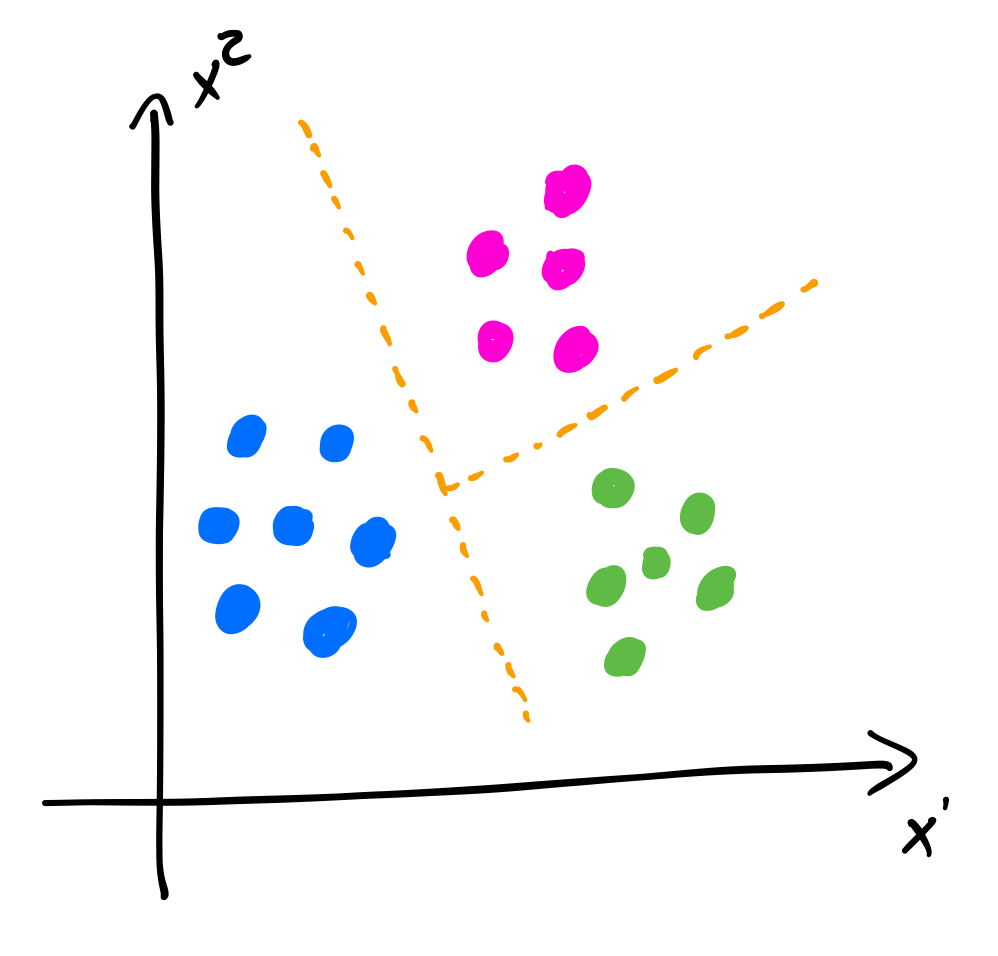
\includegraphics[scale=0.11]{./figs/Regressao_Logistica_Fig9.png}\hspace{1cm}
\end{center}
}

\Sli{Existem algumas abordagens para tratar esse problema, tais como OVO (\emph{one-versus-one}) e OVA (\emph{one-versus-all}). Vamos considerar a abordagem OVA. Neste caso, para um problema de classificação com $c$ classes, temos que criar $c$ classificadores. Vejamos o exemplo abaixo em que $c=3$.

\begin{center}
\begin{tabular}{ccc}
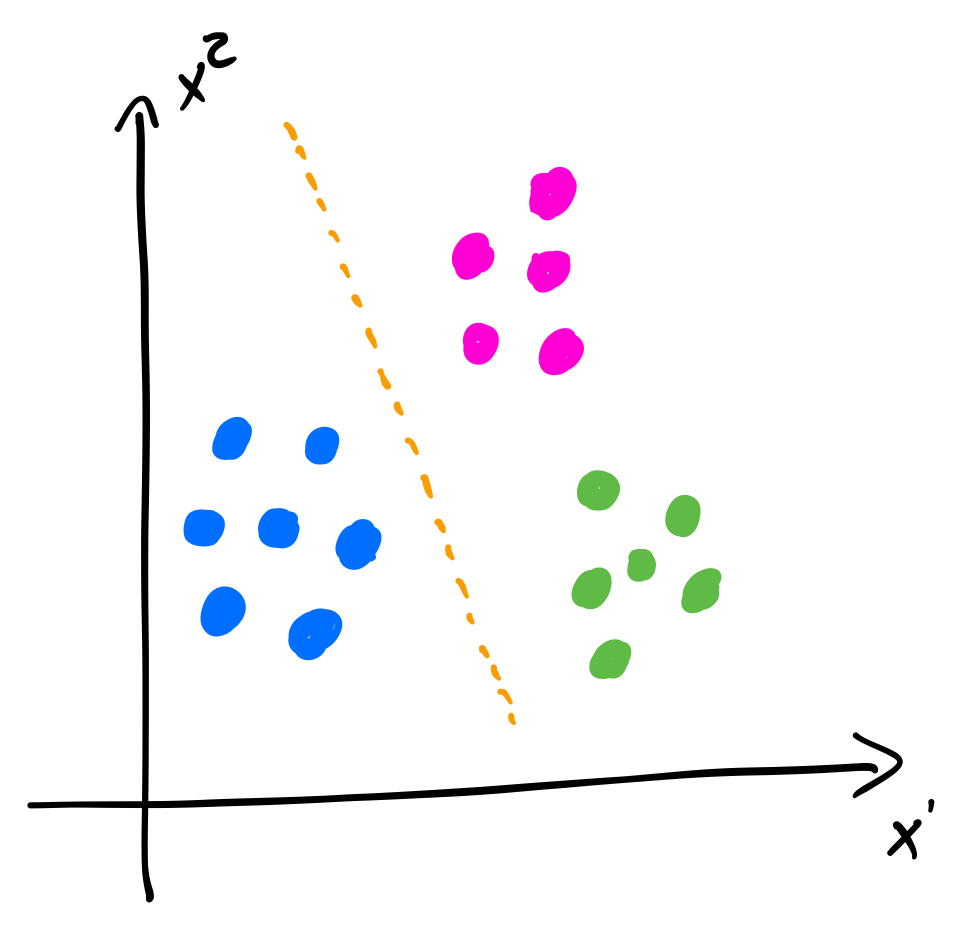
\includegraphics[scale=0.11]{./figs/Regressao_Logistica_Fig10.png} &
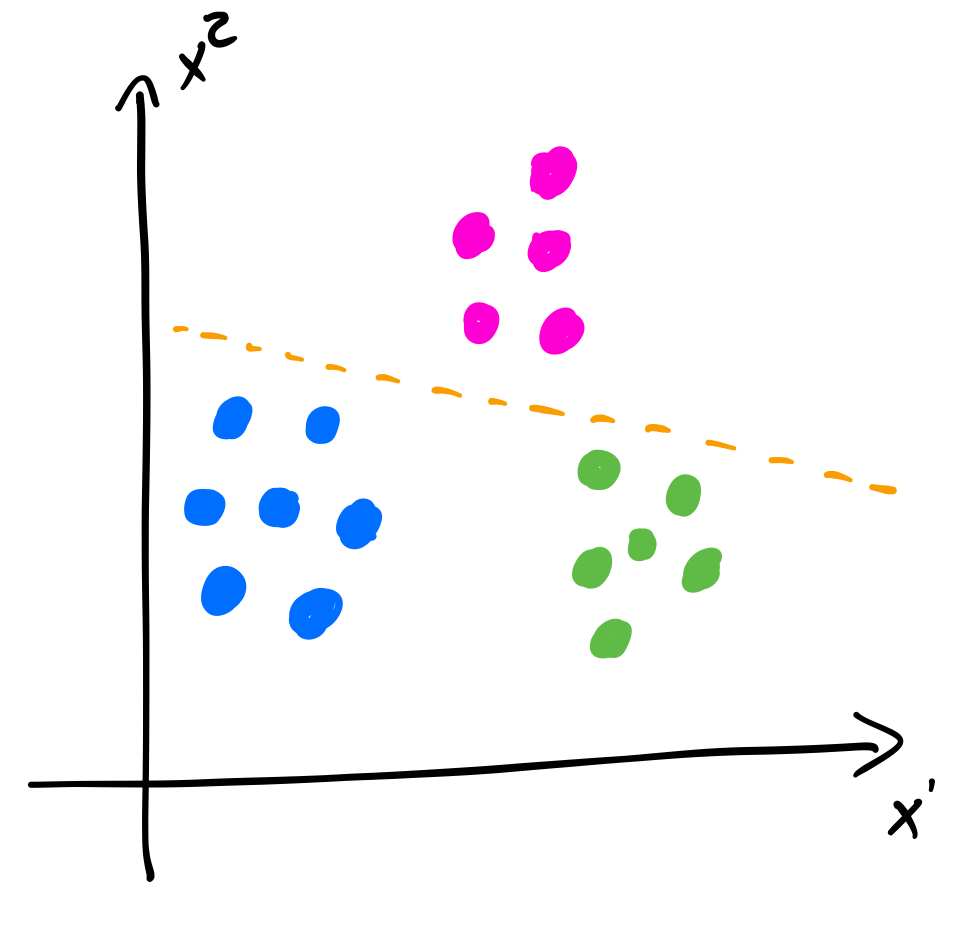
\includegraphics[scale=0.11]{./figs/Regressao_Logistica_Fig11.png} &
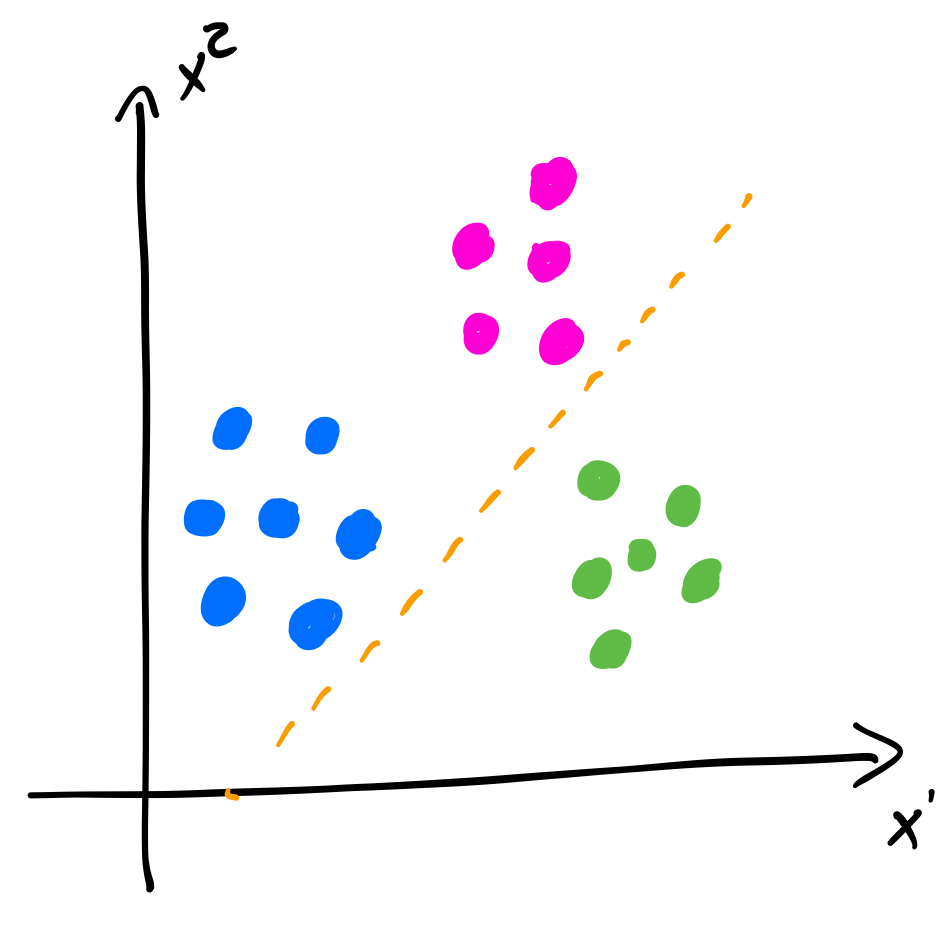
\includegraphics[scale=0.11]{./figs/Regressao_Logistica_Fig12.png} \\
Azul versus todos & Rosa versus todos & Verde versus todos \\
$h^1_{\boldsymbol{w}}(\boldsymbol{x})$ & $h^2_{\boldsymbol{w}}(\boldsymbol{x})$ & $h^3_{\boldsymbol{w}}(\boldsymbol{x})$
\end{tabular}
\end{center}
}

\Sli{
Basta, então, treinarmos cada classificador $h^i_{\boldsymbol{w}}(\boldsymbol{x})$, $\forall i = 0,1,\ldots,c-1$ em ${\cal X}^1$. Dada uma amostra $\boldsymbol{x}\in{\cal X}^2$, seu rótulo $y$ será aquele que obedece à seguinte regra de decisão:

\begin{equation}
	y = \argmax_{i}\{h^i_{\boldsymbol{w}}(\boldsymbol{x})\}.
\end{equation}
}

\SliT{Regularização}{
\justify Como vimos anteriormente, a ideia da regularização é evitar com que a técnica fique muito \textbf{especializada} (viciada) no conjunto de treinamento e, portanto, não consiga generalizar muito bem no conjunto de teste. Vejamos as três principais situações que podem ocorrer em classificadores de padrões.

\begin{center}
\begin{tabular}{ccc}
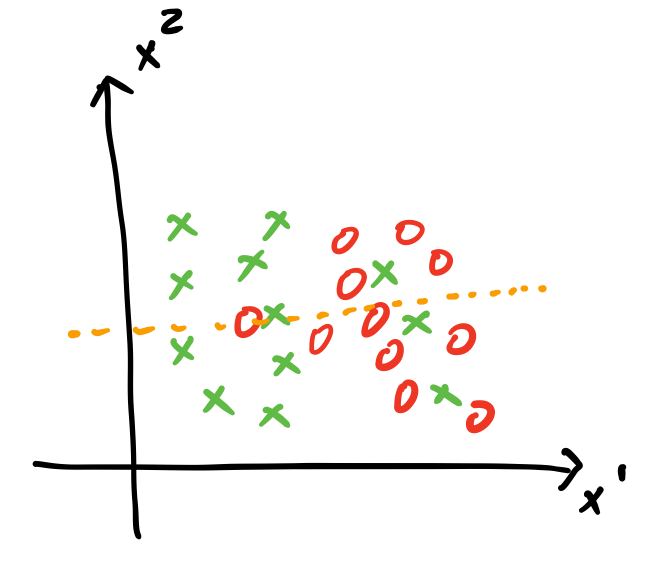
\includegraphics[scale=0.17]{./figs/Regressao_Logistica_Fig13.png} &
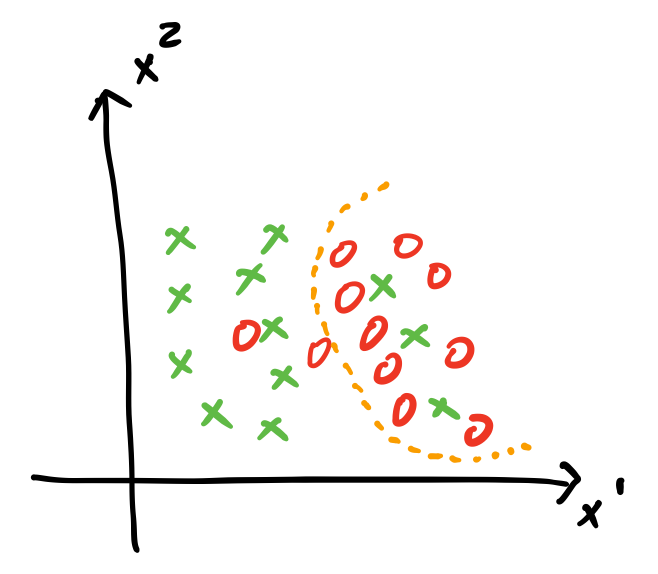
\includegraphics[scale=0.17]{./figs/Regressao_Logistica_Fig14.png} &
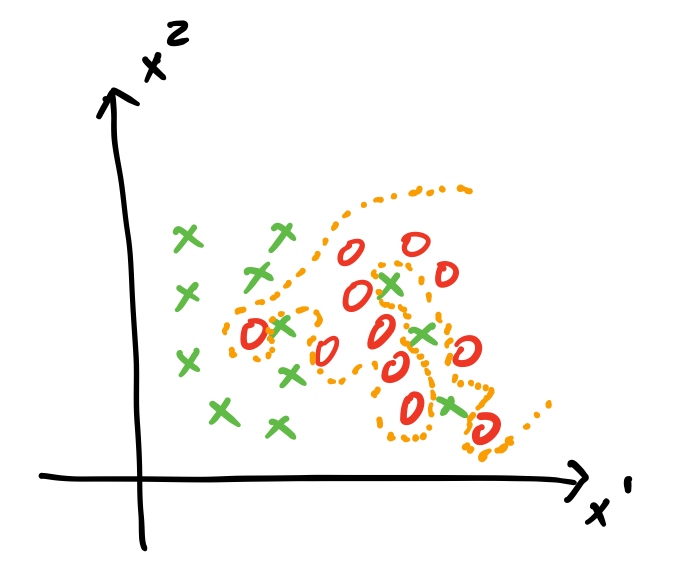
\includegraphics[scale=0.17]{./figs/Regressao_Logistica_Fig15.png} \\
Subtreinamento & Bom treinamento & Supertreinamento \\
\end{tabular}
\end{center}
}

\Sli{
Com isso, podemos modificar a Equação 5 da função de custo como segue:

\begin{equation}
	J(\boldsymbol{w}) = \frac{1}{m} \sum_{i=1}^m[-y_i\log(h_{\boldsymbol{w}}(\boldsymbol{x_i}))-(1-y_i)\log(1-h_{\boldsymbol{w}}(\boldsymbol{x}_i))]+\frac{\lambda}{2m}\sum_{j=1}^nw^2_j,
\end{equation}
em que $\lambda$ corresponde à taxa de regularização. Já as derivadas parciais da nova função de custo equivalem à derivadas da MSE no caso da regressão linear, como segue:

\begin{equation}
	\frac{\partial J(\boldsymbol{w})}{\partial w_0} = \frac{1}{m}\sum_{i=1}^m(h_{\boldsymbol{w}}(x_i)-y_i),
\end{equation}
e
\begin{equation}
	\frac{\partial J(\boldsymbol{w})}{\partial w_j} = \frac{1}{m}\sum_{i=1}^m[(h_{\boldsymbol{w}}(x_i)-y_i)x_i^j]+\frac{\lambda}{m}w_j.
\end{equation}
O algoritmo do gradiente descendente permanece o mesmo.
}

\end{document}